\problemname{Mineralfund}

\illustration{.3}{img/turnbull.jpg}{Eroderende muddervæg, der afslører nye mineraler. Foto: Michael D. Turnbull, licens: CC BY-SA.}

\noindent
Du håndterer signalbehandlingen for et rumfartsselskab,
der udvinder mineraler på fjerne himmellegemer.
Dit rumskib nærmer sig i øjeblikket en asteroide.
Indledende skanninger viser tilstedeværelsen af $k$~mineralforekomster på asteroiden, men deres nøjagtige positioner er ukendte.

\medskip

Vi betragter asteroidens overflade som et gitter af heltalskoordinater.
Hver af mineralforekomsterne er placeret på ukendte heltalskoordinater, 
således at den $i$'te forekomst har koordinaterne $(x_i, y_i)$, der opfylder
$-b \le x_i \le b$ og $-b\le y_i \le b$ %constraint:depositcoords
for noget heltal $b$ svarende til størrelsen af din indledende skanning.

For at bestemme de nøjagtige positioner af mineralforekomsterne kan du sende sonder til asteroidens overflade. 
Sonderne sendes ud i bølger af flere sonder ad gangen.

Når en sonde ankommer til sine koordinater, bestemmer den manhattan-afstanden til hver af de $k$ mineralforekomster og sender afstandene tilbage til rumskibet.
Alle datapakker ankommer samtidigt, og det er ikke muligt at afgøre, hvilke sonder der har returneret hvilke afstande. 
En bølge returnerer altså $k\cdot d$ heltal, der repræsenterer afstandene:
\[
|x_i-s_j| + |y_i - t_j| \qquad\text{for alle } i \in \{1,\ldots,k\} \text{ og } j \in\{ 1,\ldots,d\}\,.
\]
Du skal minimere antallet af bølger af sonder, der sendes til overfladen.

\section*{Interaktion}

Dette er et interaktivt problem.
Interaktion begynder med, at du læser en enkelt linje, der indeholder tre heltal $b$, $k$ og $w$:
gitterets begrænsning~$b$,
antallet~$k$ af mineralforekomster og
det maksimale antal~$w$ af bølger, du må sende.

Herefter kan du stille højst $w$ spørgsmål, hvert svarende til én bølge af sonder.
En spørgsmål består af \texttt{?} efterfulgt af $2d$~heltal adskilte af mellemrum, fx ``\texttt{?} $s_1$ $t_1$ $\cdots$ $s_d$ $t_d$'', hvor antallet~$d$ af sonder i denne bølge skal opfylde
$1\leq d\leq 2000$. % constraint:wavesize
Værdierne $(s_i,t_i)$ bliver tolket som koordinaterne for den $i$'te sonde og skal opfylde 
$-10^8 \leq s_i \leq 10^8$ og $-10^8 \leq t_i \leq 10^8$. % constraint:probecoordinates
Svaret, du får tilbage, er en enkelt linje med $k \cdot d$~heltal i ikke-aftagende rækkefølge:
manhattan-afstande mellem alle par af mineralforekomster og sondekoordinater.
Det samlede antal sonder på tværs af alle bølger må ikke overstige
$2\cdot 10^4$. % constraint:totalprobes

Interaktionen afsluttes med, at du skriver en enkelt linje bestående af \texttt{!} efterfulgt af $k$ punkter $x_1, y_1, x_2, y_2,$ $\ldots,$ $x_k, y_k$, adskilte af mellemrum.
Dette skal være den sidste linje, du skriver.

Din indsendelse bedømmes som korrekt, hvis du har skrevet de korrekte positioner for samtlige mineralforekomster.
Du kan skrive dem i vilkårlig rækkefølge.


\section*{Begrænsninger  og pointgivning}

Der gælder altid
$1\leq b \leq 10^8$, % constraint:b
$1 \leq k \leq 20$, % constraint:k
og
$2 \le w \leq 10^4$. % constraint:w

Din løsning vil blive testet på en række testgrupper, hver med en vist antal point.
Hver testgruppe indeholder en række testfald.
For at opnå point for en testgruppe skal du løse alle testfald i testgruppen.
Din endelige score vil være den højeste score for en enkelt indsendelse.

\medskip
\begin{tabular}{lll}
Gruppe & Point & Begrænsninger \\\hline
$1$ & $9$ & $k = 1, w = 10^4$, $b \le 10^7$\\
$2$ & $19$ & $w \ge 500$, $b \le 10^7$\\
$3$ & $11$ & $w \ge 210$, $b \le 10^7$\\
$4$ & $7$ & $w \ge 130$, $b \le 10^7$\\
$5$ & $20$ & $w \ge 3$, $b \le 10^4$\\
$6$ & $15$ & $w \ge 3$, $b \le 10^7$\\
$7$ & $19$ & \emph{Ingen yderligere begrænsninger}
\end{tabular}

\section*{Eksempel}

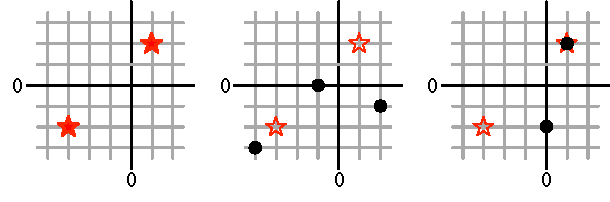
\includegraphics[width=.6\textwidth]{img/sample1.pdf}

I dette eksempel er der $k=2$~mineralforekomster på positionerne $(1,2)$ og $(-3,-2)$, vist som røde stjerner.
I den første bølge kan du måske sende $d=3$ sonder til $(-4,-3)$, $(-1, 0)$ og $(2,-1)$, vist som sorte prikker.
Denne bølge ville returnere de $6$ afstande \[
  2, 4, 4, 4, 6, 10\,.
\]
I næste bølge ville du måske sende $d=2$~sonder til $(1,2)$ og $(0,-2)$.
Denne bølge ville returnere de $4$ afstande
\[
  0, 3, 5, 8\,.
\]
